I dette kapitel beskrives implementeringen af app'en, der omhandler tranformationen fra design til kode. Dette vil være med udgangspunkt i designklasserne for henholdsvis grænseflade, model og controller. Hertil vil databasen samt kommunikation med denne indrages for således at give et indblik i, hvordan dette er implementeret. Ydermere vil de centrale elementer i app'en beskrives. Disse elementer omhandler tilpasning af træningsniveau samt resultater for brugeren. Overordnet vil beskrivelserne tage udgangspunkt i udpluk af den implementeret kode.

I \autoref{cha:design} er analyse- og designklasser samt funktionsnavne navngivet på dansk, hvorfor bogstaverne æ, ø og å forekommer. Disse symboler anvendes ikke under implementeringen for at undgå fejl.

\section{Android Studio}
Det er valgt at implementere app'en i Android Studio version 2.3.1 og programmere i Java, da dette er et objektorienteret programmeringssprog \citep{Brahma2015}. Android Studio er et officelt Integrated Development Environment (IDE) for udvikling af android app's \citep{android2017}.

Strukturen i Android Studio opdeles i Manifests, res samt java mappe. Manifests mappen indeholder en \textit{AndroidManifest.xml} fil, der er essentiel for, at app'en kan køre og indeholder aktiviter, der er implementeret. I manifestet er der derudover defineret tilladelser for den givne app. Dette kan eksempelvis være tilladelse til brug af internet samt GPS, der har været nødvendigt for at kunne tilgå databasen og beregne afstand i relation til konditionstræningen. 
Res mappen indeholder ikke-kode ressourcer, der eksempelvis er de forskellige layouts.
Javaklasserne, der er oprettet i forbindelse med udviklingen af app'en er placeret i java mappen.\citep{android2017}
 

\section{Implementering af grænseflader}
Til at implemtere boundary klasserne i systemet benyttes XML-filer, der håndteres i deres respektive controllere. I disse filer er det muligt at definere, hvilke type elemtenter, der skal indgå i layoutet. Dertil kan typen af layout defineres alt efter, hvordan layoutet skal opstilles. Layouts brugt i dette system er af type linear og relativ layout.  

Elementer opstilles i layouts med type, størrelse samt orientering. Forekommer det, at elementerne skal benyttes i javakoden, defineres disse ligeledes med et id. Et eksempel af layoutkode fra log ind ses af \autoref{fig:logindlay}.

\begin{figure} [H]
\centering
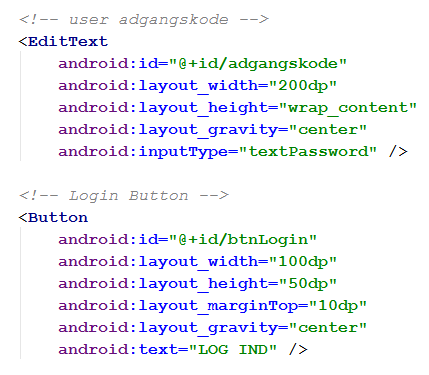
\includegraphics[width=0.6\textwidth]{figures/imple/logindlay}
\caption{Udklip af kode fra log ind layout. Udklippet viser et \textit{EditText}, hvori brugeren angiver adgangskode samt en button for log ind.}
\label{fig:logindlay}
\end{figure}

\noindent
Af dette udklip ses koden for tekstfeltet, hvori brugeren angiver adgangskode samt koden for layoutet af log ind-knappen. Feltet for adgangskoden er her af typen \textit{EditText}, der tillader, at brugeren kan angive tekst. Dette felt har ligeledes et id, der muliggører at referere til feltet og hente den angivet adgangskode til validering af log ind. Knappen er opstillet af typen button, og har ligeledes et id, hvortil en listener er opstillet i javakoden, hvilket beskrives af \autoref{sec:impmodelcon} 

\section{Implementering af model og controller klasser} \label{sec:impmodelcon}
Model og controllerklasser er implementeret i \textit{Java Class} filer. Heri er klasser defineret med navn samt tilhørende antributter og metoder. Af \autoref{fig:javaclass} ses et eksempel på, hvordan en controller er implementeret. 

\begin{figure} [H]
\centering
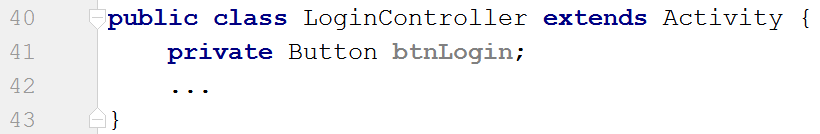
\includegraphics[width=0.6\textwidth]{figures/imple/javaclass}
\caption{Et udpluk af javaklassen for LoginController.}
\label{fig:javaclass}
\end{figure}

Det fremgår af dette udklip, at klassen er af typen public og nedarver \textit{activity}. Dette gør sig gældende for samtlige klasser implementeret. Denne klasse for \textit{LoginController} har atributten \textit{btnLogin}, der referer til log ind knappen på grænsefladen. Idet app'en skal reagerer, når brugeren trykker på btnLogin opsættes en listener på knappen, hvilket ses af \autoref{fig:list}.

\begin{figure} [H]
\centering
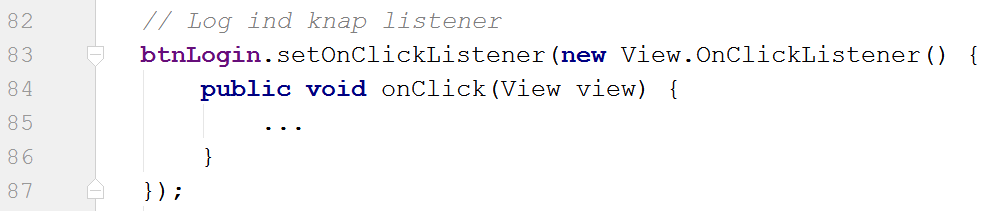
\includegraphics[width=0.6\textwidth]{figures/imple/list}
\caption{Et udpluk af listeneren opsat for log ind knappen.}
\label{fig:list}
\end{figure}

Af dette udklip ses den opsatte listener, der har til formål at lytte på knappen. Indenfor listeneren er der opstillet kode, der køres idet der trykkes på knappen. Denne listener er implementeret for samtlige knapper i controllerklasserne, da det er disse klasser, der håndterer input for tilhørende layouts. 

Modelklasserne er implementeret på samme vis som controller klasserne, de har dog til formål at lagre data forinden det sendes til databasen. Der er ligeledes opstillet attributter i modelklasserne med tilhørende get og set metoder. 

